%%%%%%%%%%%%%%%%%%%%%%%%%%%%%%%%%%%%%%%%%%%%%%%%%%%%%%%%%%%%%%%%%%% 
%                                                                 %
%                            CHAPTER                              %
%                                                                 %
%%%%%%%%%%%%%%%%%%%%%%%%%%%%%%%%%%%%%%%%%%%%%%%%%%%%%%%%%%%%%%%%%%% 

\chapter{Achtergrond}

\section{Fitnesstrackers}
De focus van deze scriptie ligt op mogelijke tekortkomingen of vulnerabilities
betreffende het privacybeleid in fitnesstrackers. Maar vooraleer we een aanval
op basis van deze kwetsbaarheden kunnen opzetten, is het noodzakelijk om een
vat te krijgen op welke manier een fitnesstracker info verzamelt en weergeeft,
en meer precies, hoe de mechanismen die de privacy voorzien voor de gebruikers
in detail werken.

De data waarmee de aanval wordt opgezet en waarmee wordt geëxperimenteerd, is
afkomstig van de populaire fitnesstracker
\textit{Strava\footnote{\url{https://www.strava.com/}}}. Dit is een sociaal
netwerk waarbij alle soorten sporters hun activiteiten kunnen delen. Dit gaat
over lopen, wandelen, fietsen, zwemmen, maar ook sporten als fitnessen,
voetballen, etc. De verzamelde data wordt volgens het perspectief van een
mogelijke aanval gefilterd, niet alle data blijkt nuttig te zijn. Enkel data
die gevoelige informatie met betrekking tot de woonplaats zou kunnen vrijgeven
wordt behouden. Dit zal er dus op neerkomen dat enkel activiteiten die
relevante \ac{gps}-informatie bevatten in beschouwing worden genomen, meer
specifiek zal dit gaan over \textit{runs, hikes, walks, and rides}.

\subsection{Activiteiten}\label{data}
Een Strava-activiteit bevat erg veel informatie. Echter is niet alles even
bruikbaar. Een correcte abstractie van de onnodige data is dus nodig.
Figuur~\ref{fig:activityData} geeft een voorbeeld van een gedetailleerde
activiteit weer. Een gebruiker is in staat om de activiteit een titel te geven,
en er een korte beschrijving aan toe te voegen. Ook een foto kan optioneel
toegevoegd worden. De exacte datum en tijd van de start van de activiteit wordt
hierbij ook weergegeven.

Rechts bovenaan zijn de algemene basisstatistieken te zien. Dit zijn de totale
afgelegde afstand, de totale bewegingstijd, de gemiddelde snelheid of het
gemiddelde tempo, het totale hoogteverschil, de totale verstreken tijden, en
het aantal calorieën verbrand. Als extra kunnen hier enkele statistieken
m.b.t.\ het gebruikte materiaal, zoals type fiets, loopschoenen, hartslagmeter,
enzovoort worden weergegeven. Een belangrijk onderscheid in deze context is het
verschil tussen de beweegtijd en de verstreken tijd. Deze twee lijken in
definitie gelijk, maar dit zijn ze niet. Strava, en fitnessplatformen in het
algemeen werken met twee verschillende soorten tijdsberekeningen voor het
bekomen van een accuratere gemiddelde snelheid of tempo. De verstreken tijd is
simpelweg het tijdsinterval tussen het vertrek van de activiteit en de
aankomsttijd ervan. De bewegingstijd is de tijd waarbij de gebruiker zich
effectief bewoog. Met andere woorden worden de tijden waarbij de gebruiker
stilstond uit de verstreken tijd gefilterd. Dit kan gaan over bijvoorbeeld een
pauze, of het wachten voor een verkeerslicht.

Er is een verschil bij fietsactiviteiten en wandelactiviteiten in hun weergave.
In het geval van een fietsactiviteit wordt \textit{snelheid} weergegeven, en in
het geval van een wandel- of loopactiviteit wordt \textit{tempo} weergegeven,
zoals te zien is op Figuur~\ref{fig:speedvspace}. Deze worden beide berekend
aan de hand van de bewegingstijd. Een kanttekening hierbij is dat dit enkel
geldt voor activiteiten die niet gelabeld zijn als \textit{race}, indien dit
toch het geval is, wordt de snelheid berekend in functie van de totaal
verstreken tijd~\cite{MovingTi80:online}. Het verschil tussen deze twee is dat
de snelheid wordt berekend volgens de formule $ \quad v = \frac{d}{t}$. De
eenheid van snelheid is dan ook $\frac{m}{s}$ of, in het geval van
fitnesstrackers, $\frac{km}{h}$. Het tempo wordt berekend volgens de formule $
    \quad tempo(\frac{\min}{km}) = \frac{t(\min)}{d(km)}$. De eenheid van tempo is
$\frac{\min}{km}$. Om deze berekeningen wat te standaardiseren, werd gedurende
deze thesis gekozen om altijd de omrekening te maken naar snelheid
$\frac{km}{h}$, om zo over de volledige lijn met dezelfde standaard te werken.
\begin{figure}[h]
    \centering
    \begin{subfigure}[b]{.5\textwidth}
        \centering
        \caption{Voorbeeldroute zonder map snapping}
        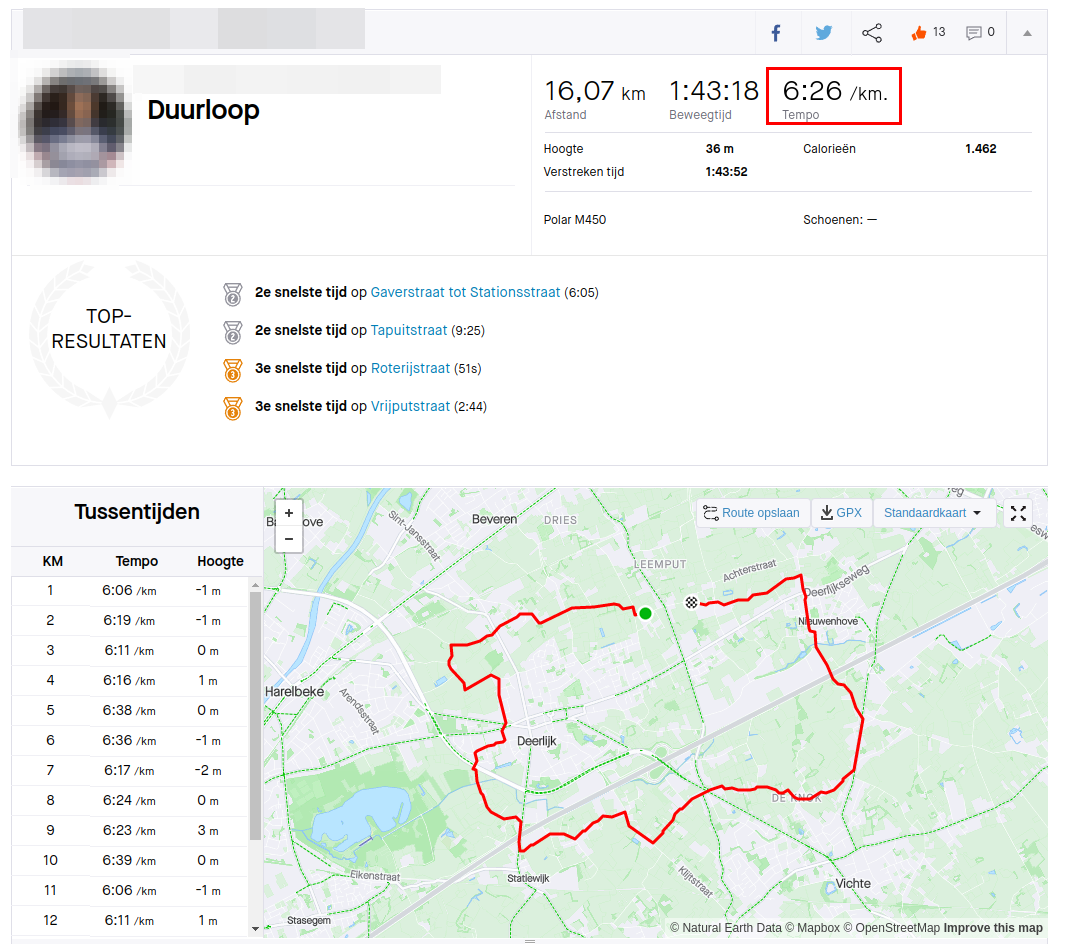
\includegraphics[width=\textwidth]{fig/SpeedVSPace/Pace.png}
    \end{subfigure}\hfill
    \begin{subfigure}[b]{.5\textwidth}
        \centering
        \caption{Fietsrit gebruikt snelheid}
        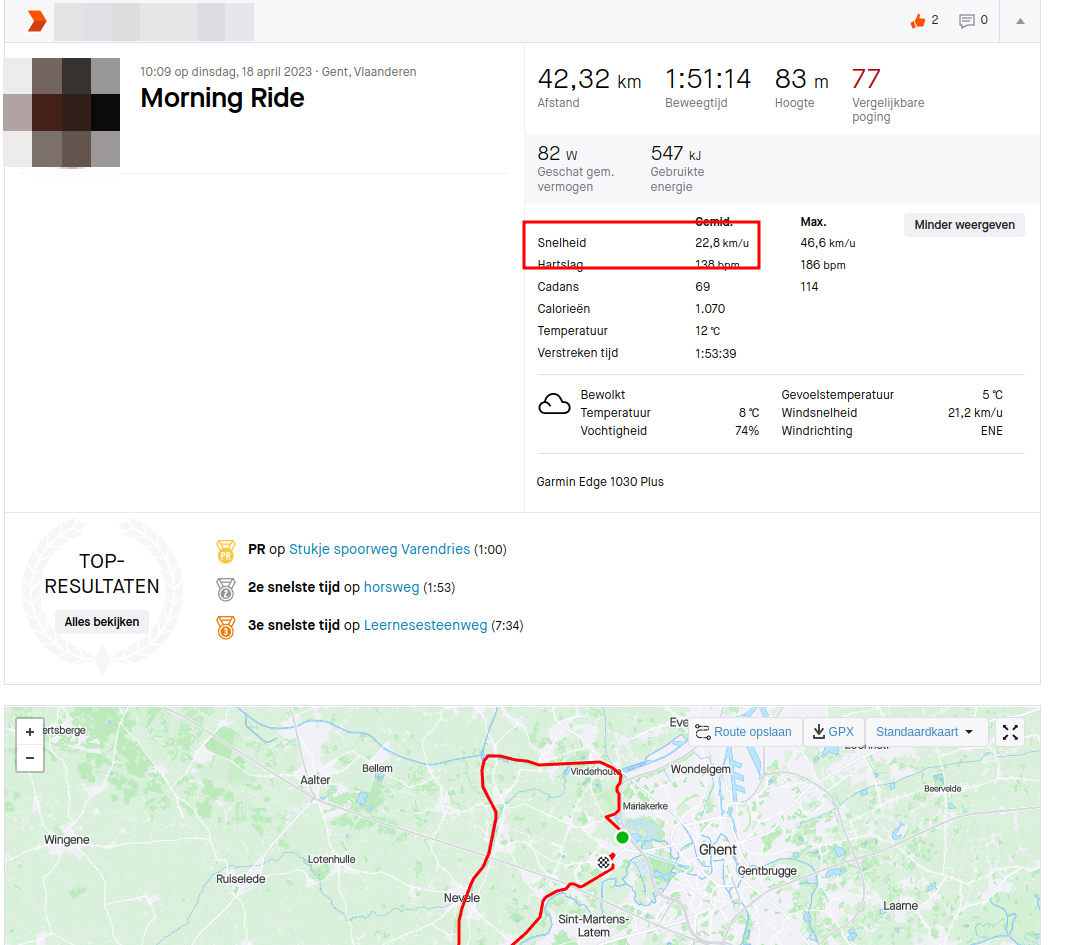
\includegraphics[width=\textwidth]{fig/SpeedVSPace/Speed.png}
    \end{subfigure}
    \caption{Verschil snelheid en tempo}\label{fig:speedvspace}
\end{figure}

Onder de basisstatistieken zijn de \textit{Strava-segmenten} te zien. Een
Strava-segment is een specifiek deel van een bepaalde route dat gebruikers van
de sport-app kunnen markeren, delen en vergelijken met andere gebruikers. Het
segment is een bepaalde afstand en route, bijvoorbeeld een klim of afdaling,
die vaak wordt beschouwd als een uitdagende of iconische sectie van een
bepaalde fiets- of hardlooproute. Gebruikers van Strava kunnen een segment
maken door de begin- en eindpunten op een kaart aan te geven en een naam en
beschrijving toe te voegen. Zodra het segment is gemaakt, kunnen andere
gebruikers het segment vinden en deelnemen aan een leaderboard, waarop de
snelste tijden worden bijgehouden en vergeleken met andere gebruikers.
Segmenten worden vaak gebruikt om prestaties te meten en te vergelijken.

Centraal op de figuur is ook de kaart duidelijk zichtbaar. Daarbij horen ook de
tussentijden en de grafiek van de snelheidsevolutie. Optioneel kan hierbij ook
nog een visualisatie van de afgelegde hoogte en de hartslag worden weergegeven,
indien de gebruiker hiervoor met de juiste meetinstrumenten zijn
sportactiviteit opneemt. De tussentijden en de grafiek van snelheid zijn qua
inhoud gelijkaardig, met als verschil dat de waarden op de grafiek erg precies
kunnen worden bestudeerd. Op de grafiek is voor elk afstandspunt de
ogenblikkelijke snelheid zichtbaar. Bij de tussentijden wordt de gemiddelde
snelheid over een kilometer weergegeven. De kaart die de route weergeeft is
zeker ook belangrijk om even te bestuderen. Deze bevat namelijk alle
\ac{gps}-geregistreerde punten, en verbindt deze ook om zo één aaneensluitende
route te vormen. Wanneer deze echter in detail bestudeerd wordt, samen met de
legende die aanwezig is, is te zien dat de route uit twee delen bestaat, een
zichtbaar deel en een onzichtbaar deel. Een andere gebruiker zal enkel zicht
hebben op het zichtbare deel, het onzichtbare deel zal dus voor een andere
gebruiker niet zichtbaar zijn. Anders geformuleerd, de activiteit zal voor deze
persoon dus als het ware afgekapt zijn, en zal in de voor hem of haar zichtbare
versie op een andere plek starten en eindigen. In de volgende
Secties~\ref{sec:Algemene Privacy} \&~\ref{sec:EPZ} wordt meer in detail
ingegaan op de werking van deze methodiek.

Een laatste kanttekening die we hierbij maken, is dat een gebruiker keuze heeft
tussen verschillende eenheden. Er is keuze mogelijk tussen de mijl en pond, en
kilometer en kilogram. Gebruikers kiezen in welke eenheid ze de applicatie
wensen te gebruiken. Voor de gebruiker in kwestie zal dan ook de volledige
applicatie worden weergegeven in de gekozen eenheden.
\begin{figure}
    \centering
    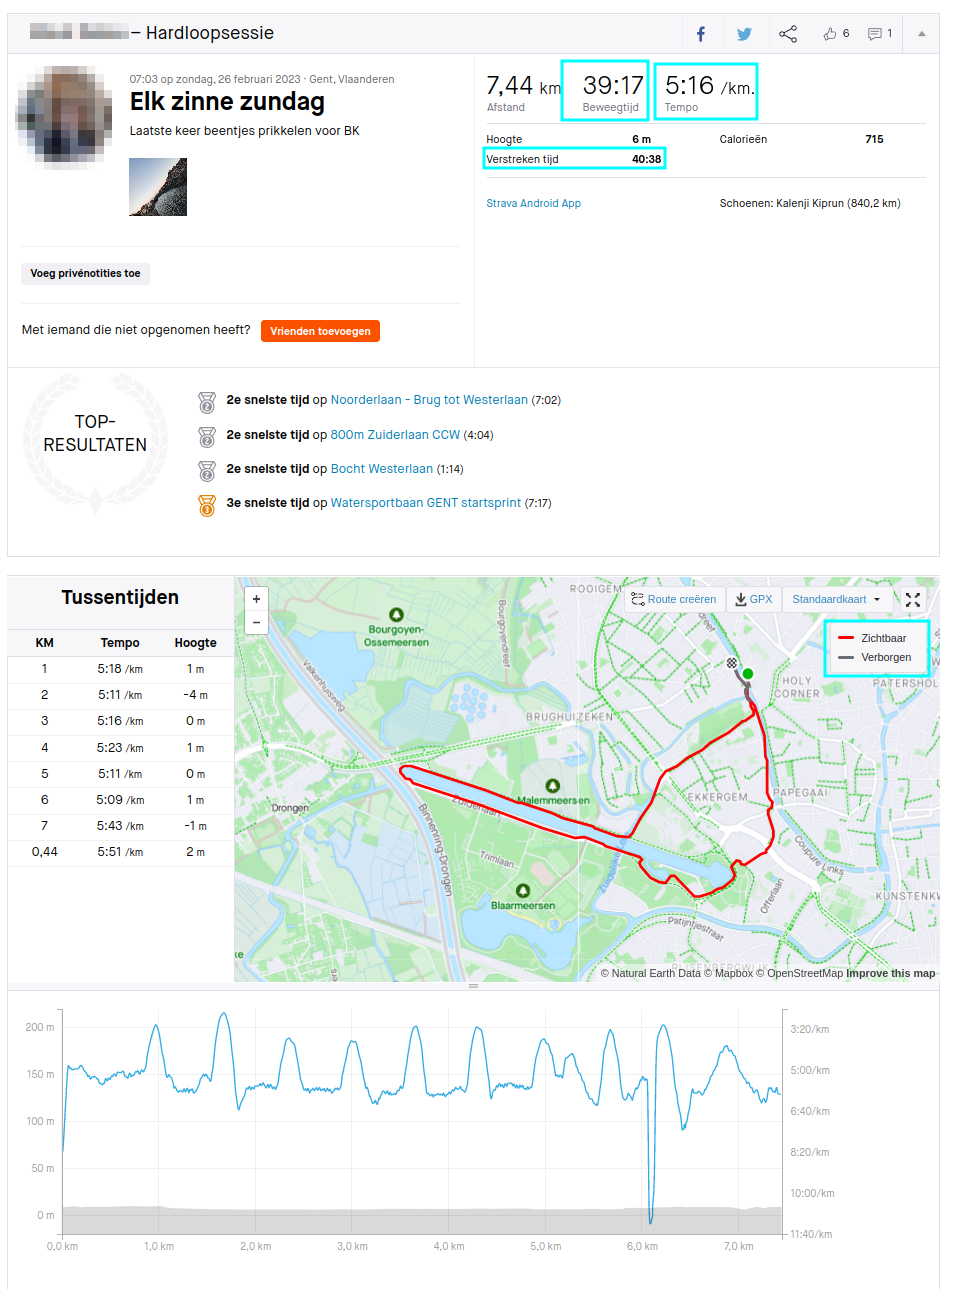
\includegraphics[width=0.8\textwidth]{fig/VoorbeeldActiviteiten/VoorbeeldActiviteit_Personal.png}
    \caption{Data van een activiteit}\label{fig:activityData}
\end{figure}

\subsection{Berekening Afstanden}\label{sec:afstandsberekeningen_strava}
Fitnesstrackers krijgen vanuit de buitenwereld ruwe data binnen. Deze data moet
dus verwerkt worden vooraleer ze bruikbaar is voor de gebruiker. Er werd al
kort ingegaan in Sectie~\ref{data} op de berekening die Strava gebruikt voor de
snelheid. Echter is het ook interessant om de berekening van Strava eens onder
de loep te nemen voor de afgelegde afstand. Strava maakt gebruik van twee
verschillende methodieken voor het berekenen van deze afstand. De eerste is de
\textit{GPS-calculated Distance}. Dit bestaat eruit om de afstand tussen
opeenvolgende ontvangen \ac{gps}-punten te berekenen, en deze op te tellen.
Precisie is hier afhankelijk van de precisie van de \ac{gps}-punten, aangezien
de afstand wordt berekend door de punten met rechte lijnen te verbinden. Dit
kan gebeuren in real time, via de gsm, smartwatch of ander toestel die gebruikt
wordt om de activiteit op te nemen. Er zal dan ook mogelijkheid zijn om real
time info te zien. Op elk punt zal de afstand vanaf het startpunt gekend zijn,
en het is deze afstand die gedeeld zal worden op het platform. Het grote nadeel
hierbij is het real-time aspect. Fouten kunnen moeilijker on the fly worden
gecorrigeerd. Een tweede aanpak voor GPS-calculated distance is om
\ac{gps}-data pas bij het uploaden te verwerken. De \ac{gps}-data wordt dan
geanalyseerd, en de nodige berekeningen worden uitgevoerd.

Het alternatief voor de GPS-calculated distance is de \textit{Ground Speed
    Distance} methodiek. Deze afstand kan enkel worden bepaald in het geval van een
fietsactiviteit met behulp van een capabele fietscomputer die omwentelingen van
de wielen kan meten. De fietscomputer berekent dan de afstand door het aantal
omwentelingen te vermenigvuldigen met de omtrek van het
fietswiel~\cite{HowDista47:online}.

De bovenstaande afstandsberekeningen zijn de twee technieken die de officiële
supportdocumentatie van Strava beschrijft~\cite{HowDista47:online}. Echter
blijkt wanneer we de afstand op deze manier manueel berekenen, we afwijkende
resultaten bekomen worden. Dit is zeer waarschijnlijk te wijten aan de
preprocessing van de data die gebeurt bij het uploaden van een activiteit.
Alhoewel dit niet expliciet gedocumenteerd staat doen de resultaten dit wel
sterk vermoeden. De hypothese is dat tijdens het uploaden, de afstand
herberekend wordt. De \ac{gps}-punten zullen worden geanalyseerd, en dat het
platform hierbij technieken gebruikt om de resultaten hiervan te verbeteren. De
twee meest waarschijnlijke technieken zijn \textit{Map Snapping} en
\textit{Smoothing}.

Map Snapping (ook wel \textit{Map Matching} genoemd) is een techniek waarbij
\ac{gps}-punten worden verschoven naar de dichtstbijzijnde weg. Per
\ac{gps}-punt wordt gezocht naar de dichtste node op de desbetreffende
\textit{roadgraph}\footnote{De roadgraph is een wegennetwerk, omgezet in een
    graaf, bestaande uit edges en nodes. Elke weg of pad, bevat één of meerdere
    nodes, zodat een skeletstructuur ontstaat, die een abstractie van het
    wegennetwerk voorstelt~\cite{seiler2022haul}}, op Figuur~\ref{fig:MapSnapping}
is de werking ervan te zien~\cite{Snapping96:online}.
\begin{figure}[h]
    \centering
    \begin{subfigure}[b]{.5\textwidth}
        \centering
        \caption{Voorbeeldroute zonder map snapping}
        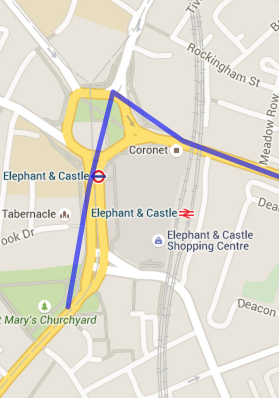
\includegraphics[width=0.5\textwidth]{fig/Map Snapping/before.png}\label{fig:before_MapSnapping}
    \end{subfigure}\hfill
    \begin{subfigure}[b]{.5\textwidth}
        \centering
        \caption{Voorbeeldroute met map snapping}
        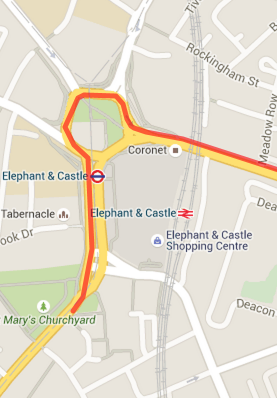
\includegraphics[width=0.5\textwidth]{fig/Map Snapping/after.png}\label{fig:after_MapSnapping}
    \end{subfigure}
    \caption{Voorbeeld van de werking van \textit{Map Snapping}~\cite{Snapping96:online}}\label{fig:MapSnapping}
\end{figure}

Daarnaast bestaat de kans dat er gebruik gemaakt wordt van smoothing. Smoothing
is een proces dat ruwe \ac{gps}-punten (of datapunten in het algemeen) op een
traject probeert te optimaliseren opdat ze een vloeiend `curve' vormen. Dit
wordt bekomen door ruis, schommelingen en onnauwkeurigheden te filteren uit het
traject. Hiervoor bestaan verschillende implementaties. Aangezien Strava geen
openbare informatie verstrekt over het gebruik van gps-smoothing, is het niet
bekend of ze deze techniek effectief toepassen. Het is dus gissen naar, indien
ze deze zouden gebruiken, welke implementatie dan wel gebruikt wordt. De
makkelijkste en meest modulaire methode om aan smoothing te doen, is
\textit{Smoothing met Moving Average}. Deze methode bestaat eruit om van een
aantal punten in een bepaalde range (ook `window' genoemd) het gemiddelde te
nemen, en vervolgens op te schuiven. Het gemiddelde wordt berekend met volgende
formule: $\overline{y_x} = \frac{y_x + y_{x+1} + \ldots + y_{x+n}}{x+n}$, voor
punt x, met n als window-grootte~\cite{Smoothin16:online,
    SmoothingandInterpolatingNoisyGPSDatawithSmoothingSplines, Smoothin86:online}.
Zo kan voor elk punt een evenwichtige waarde op de nieuwe grafiek bekomen
worden, en krijgt de grafiek een meer vloeiende vorm. Merk wel op dat de
precisie van de route afneemt op deze manier. Bij het smoothen van een traject
wordt het aantal gebruikte punten namelijk verminderd volgens de grootte van de
window. Afhankelijk van de grootte, worden meer (resp.\ minder) punten
samengenomen, en zo minder of meer punten weergegeven op de grafiek. Een
voorbeeld is terug te vinden op Figuur~\ref{fig:SmoothingExample}, waarbij de
blauwe curve de ruwe data voorstelt, dus voorafgaand op het `smoothen', en de
rode de `gesmoothe' curve.
\begin{figure}[h]
    \centering
    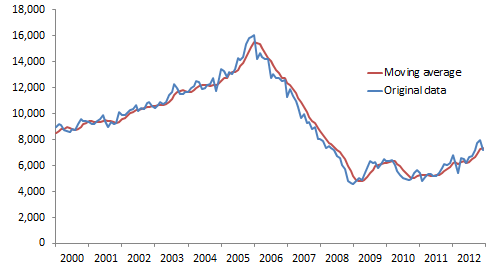
\includegraphics[width=0.6\linewidth]{fig/SmoothingExample.png}
    \caption{Voorbeeld Data smoothing met een moving average~\cite{SmoothingandInterpolatingNoisyGPSDatawithSmoothingSplines}}\label{fig:SmoothingExample}
\end{figure}

\subsection{Algemeen Privacybeleid}\label{sec:Algemene Privacy}
Het is zeker niet altijd wenselijk om alle data die vervat zit in zo'n
activiteit met alle andere gebruikers op het platform te delen. De
ontwikkelaars kiezen er dan ook voor om gebruikers de mogelijkheid te geven om
hun privacy te bewaren. In deze sectie wordt de focus gelegd op de mechanismen
gebruikt door \textit{Strava}. Er valt op dat heel wat andere sport-applicaties
vergelijkbare, zo niet dezelfde methodieken gebruiken. Een eerste algemeen
mechanisme bestaat eruit om de gebruiker de keuze te geven om alle activiteiten
en alle gegevens over het profiel heen te laten voldoen aan bepaalde privacy
regels. Deze regels kunnen ook per activiteit worden ingesteld. Onder de keuzes
staan meestal drie opties: \textit{zichtbaar voor iedereen}, \textit{zichtbaar
    voor volgers} en \textit{zichtbaar voor niemand}. Er kan ook zelfs een keuze
gemaakt worden om specifieke elementen van een activiteit niet te delen met de
buitenwereld, zoals bijvoorbeeld de zichtbaarheid van de route op de
kaart~\cite{Activity24:online}.

\section{Endpoint Privacy Zones}\label{sec:EPZ}
Een \ac{EPZ} is een cirkelvormige zone met een bepaalde straal rond een
\ac{gps}-punt. Het punt in kwestie zal dus de betreffende \textit{gevoelige
    locatie} zijn. De gebruiker kan de straal van deze cirkel\footnote{Op Strava
    heeft de \ac{EPZ} de vorm van een cirkel, maar op andere platformen kunnen
    andere vormen de norm zijn, bv.\ polygonen.} zelf kiezen, en in het geval van
Strava hebben gebruikers keuze uit waarden van 0 tot 1600m, in stappen van
200m. Wanneer een gebruiker binnen deze zone zijn activiteit beëindigt of
begint, dan zal dat deel van de route binnen de \ac{EPZ} niet zichtbaar zijn
voor anderen. Vanuit het perspectief van een andere gebruiker zal de activiteit
dus starten en/of eindigen op de rand van deze cirkel (die natuurlijk niet
zichtbaar is). Merk op dat een sporter meerdere gevoelige locaties kan
verbergen op de kaart. Bijvoorbeeld een frequent bezocht café, of een huis van
een partner waar regelmatig een tussenstop plaatsvindt. Een tweede opmerking is
dat wanneer een gebruiker de \ac{EPZ} doorkruist, maar er niet in stopt, dat
deel van de route onaangepast blijft. Op Figuur~\ref{fig:EPZ_Voorbeeld} zijn de
verschillende perspectieven te zien, hoe de eigenaar de activiteit ziet, en hoe
het eruit ziet voor een externe gebruiker. Het traject dat de buitenstaander te
zien krijgt, bestaat uit alle punten die zich buiten de \ac{EPZ} bevinden. Merk
ook op dat de eigenaar van de activiteit zicht heeft op de invloed van de
\ac{EPZ}, dus wat zal verborgen worden erdoor, en wat zichtbaar blijft. Dit
onderscheid wordt gemaakt door het verschil in kleur, oranje voor de publiek
zichtbare punten en grijs voor de onzichtbare.
\begin{figure}[h]
    \centering
    \begin{subfigure}[b]{.49\textwidth}
        \centering
        \caption{Perspectief eigenaar}
        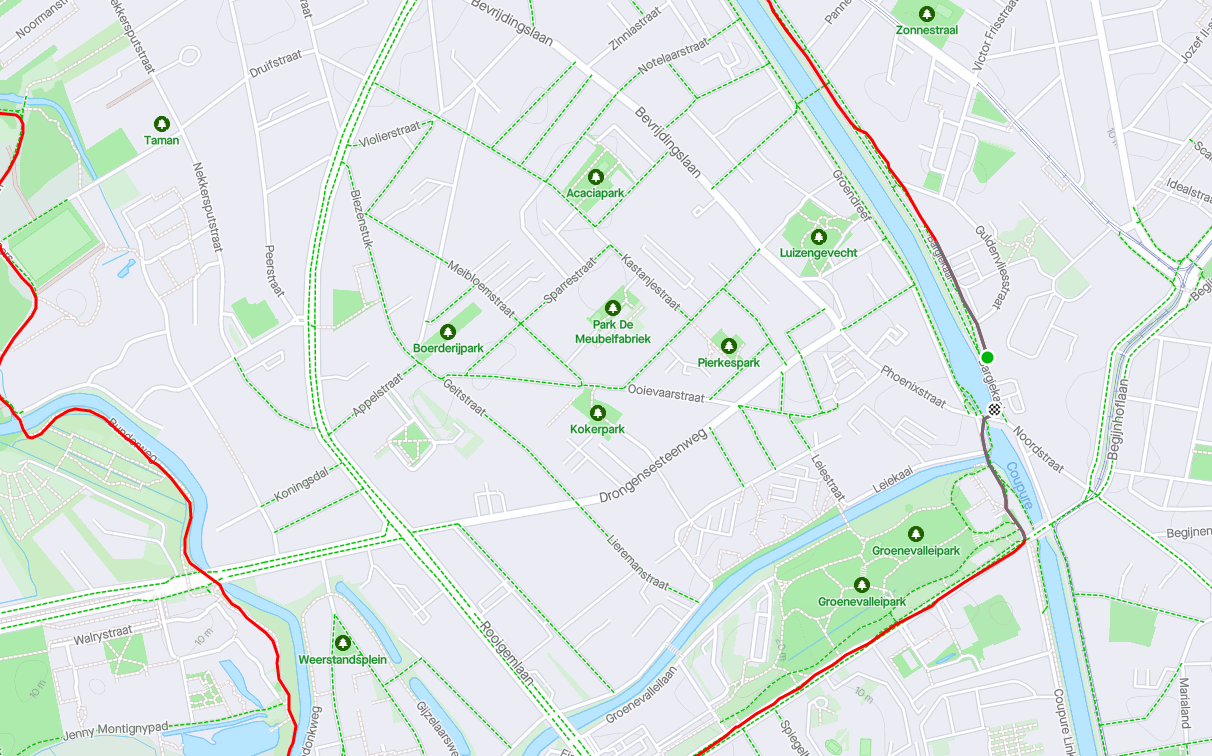
\includegraphics[width=1\textwidth]{fig/EPZ-mechanisme/Example_EPZ_InternalView.png}\label{fig:EPZ_internal}
    \end{subfigure}\hfill
    \begin{subfigure}[b]{.49\textwidth}
        \centering
        \caption{Perspectief externe gebruiker}
        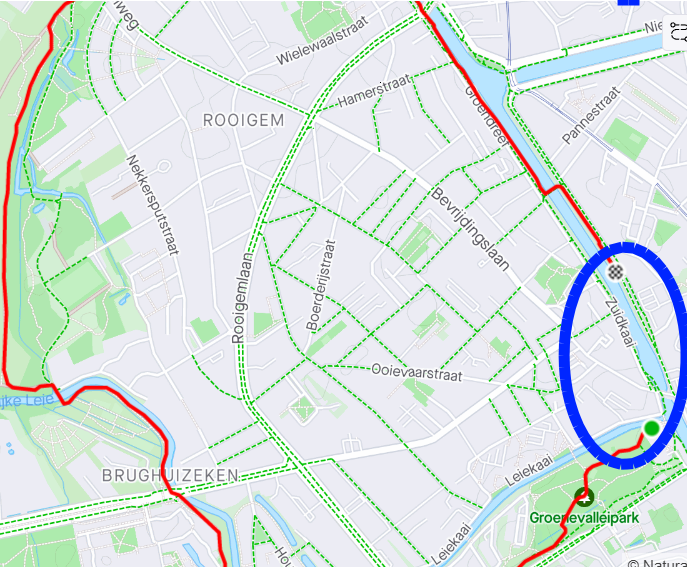
\includegraphics[width=1\textwidth]{fig/EPZ-mechanisme/Example_EPZ_ExternalView.png}\label{fig:EPZ_external}
    \end{subfigure}
    \caption{Voorbeeld van de werking van een EPZ}\label{fig:EPZ_Voorbeeld}
\end{figure}

De methodiek die fitnesstrackers toepassen bij het opzetten van een \ac{EPZ}
werkt als volgt, de gevoelige locatie wordt genomen als beginlocatie. Hieruit
zetten ze a.d.h.v.\ de op voorhand vastgelegde \ac{EPZ}-straal een cirkel op.
Het centrum van deze cirkel zal hierna een translatie ondervinden in een
willekeurige richting. Dit kan een verschuiving zijn met een afstand die
maximaal 70\% van de straal van de \ac{EPZ} bedraagt. Dit mechanisme is te zien
op Figuur~\ref{fig:translation}. Het transleren van deze cirkel wordt ook
\textit{spatial cloaking} genoemd.
\begin{figure}[h]
    \centering
    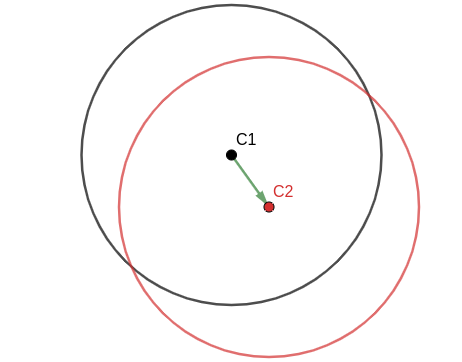
\includegraphics[width=0.4\linewidth]{fig/EPZ-mechanisme/Translation_Center.png}
    \caption{Voorbeeld translatie EPZ}\label{fig:translation}
\end{figure}

Daarna worden alle punten vertrekkende vanaf de gevoelige locatie tot aan de
rand van de \ac{EPZ}, en vanaf de rand van de \ac{EPZ} tot aan de gevoelige
locatie verwijderd van het zichtbare traject. Een voorbeeld van deze filtering
is te zien op Figuur~\ref{fig:drop points}, waarbij duidelijk zichtbaar is dat
punten die de \ac{EPZ} doorkruisen, maar niet vertrekken of aankomen bij de
gevoelige locatie niet worden gefilterd.
\begin{figure}[h]
    \centering
    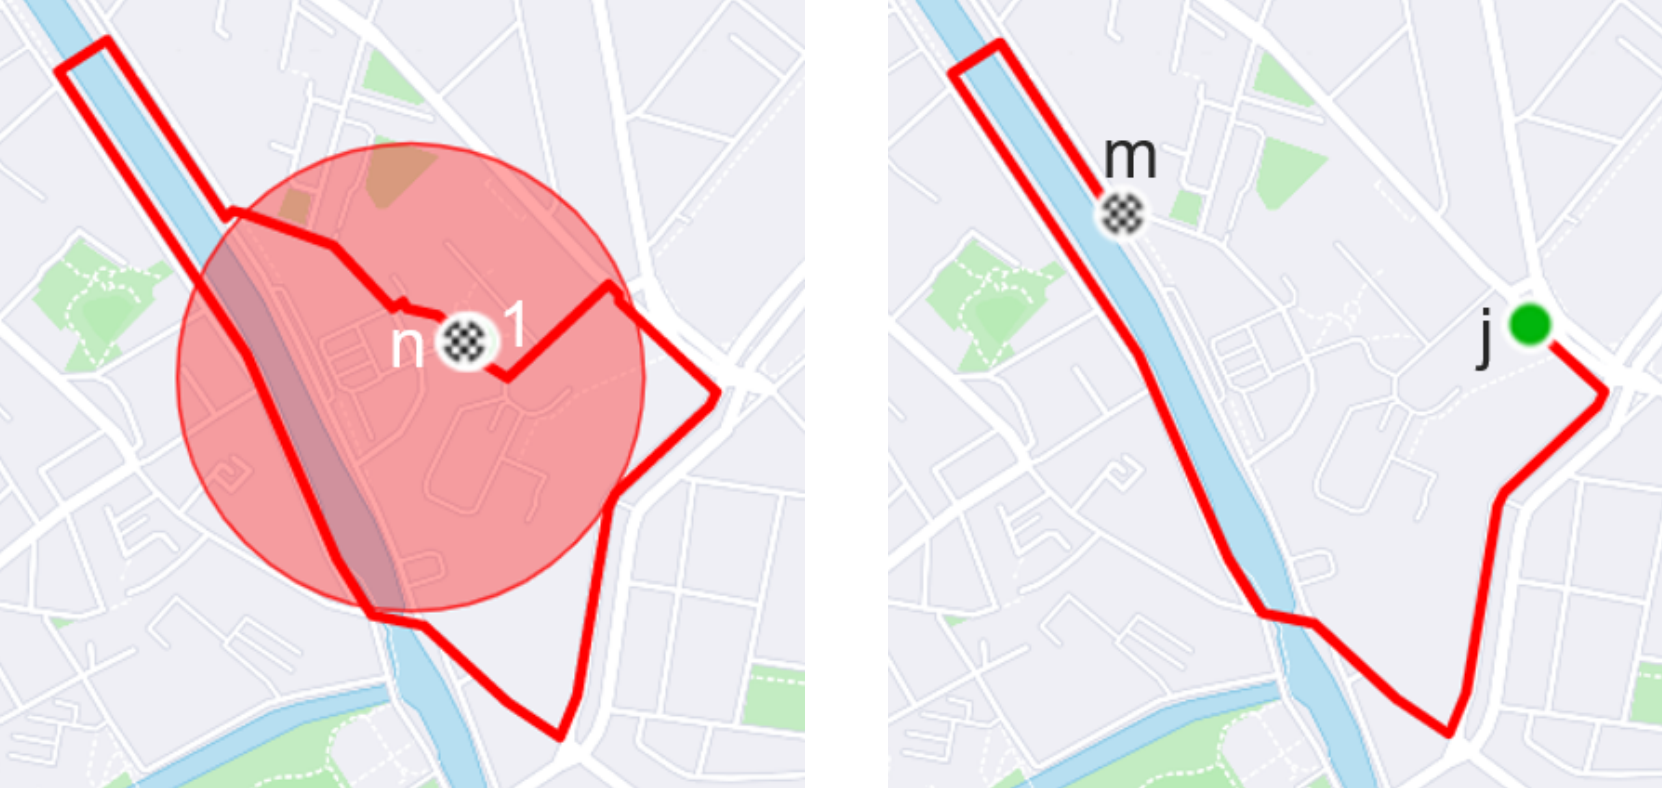
\includegraphics[width=0.7\linewidth]{fig/EPZ-mechanisme/DropEPZPoints.png}
    \caption{Voorbeeld filtering van punten binnen EPZ~\cite{Dhondt}}\label{fig:drop points}
\end{figure}

\section{Mogelijke gps-fouten}\label{sec:gps-fouten}
Zoals reeds aangehaald kunnen er bij het verzamelen van \ac{gps}-data
significante fouten optreden. Met \ac{gps}-fouten wordt gedoeld op data die de
\ac{gps}-sensor opvangt die niet overeenstemt met de werkelijke
\ac{gps}-locatie. Deze fouten kunnen verschillende oorzaken hebben. De
belangrijkste zijn hierbij \textit{\ac{gps}-drift}, \textit{\ac{gps}-signal
    loss} en \textit{\ac{gps}-bounce}.

Gps-drift is een fenomeen waarbij de \ac{gps}-locatie van een gebruiker afwijkt
van de effectieve locatie. Twee voorbeeld zijn terug te vinden op
Figuur~\ref{fig:gps_drift}, waarvan Figuur~\ref{fig:gps_drift_Strava}
rechtstreeks afkomstig is vanaf Strava. Hierbij is te zien dat de gebruiker een
deel van de route door gebouwen heen en door het water aflegt. Dit kan worden
veroorzaakt door dichtbebouwde omgevingen, en omgevingsfactoren zoals hoge
bomen. Er zijn enkele redenen waarom dit gebeurd, namelijk hoge gebouwen,
wolkenkrabbers of dichte boombedekking kunnen het GPS-signaal verstoren.
GPS-satellieten zenden radiosignalen uit die gemakkelijk kunnen worden
belemmerd of geblokkeerd door fysieke obstakels. Wanneer het signaal wordt
verstoord, kan de GPS-ontvanger moeite hebben om nauwkeurige locatiegegevens te
berekenen. Reflectie van signalen kan op zijn beurt ook een impact hebben. De
eerder beschreven map snapping kan dit eventueel tegengaan.
\begin{figure}[h]
    \centering
    \begin{subfigure}[b]{.45\textwidth}
        \centering
        \includegraphics[width=\textwidth]{fig/Afwijkingen&Analyses/Crooked Routes/GPS-drift.png}
        \caption{Voorbeeld van gps-drift op Strava}\label{fig:gps_drift_Strava}
    \end{subfigure}\hfill
    \begin{subfigure}[b]{.49\textwidth}
        \centering
        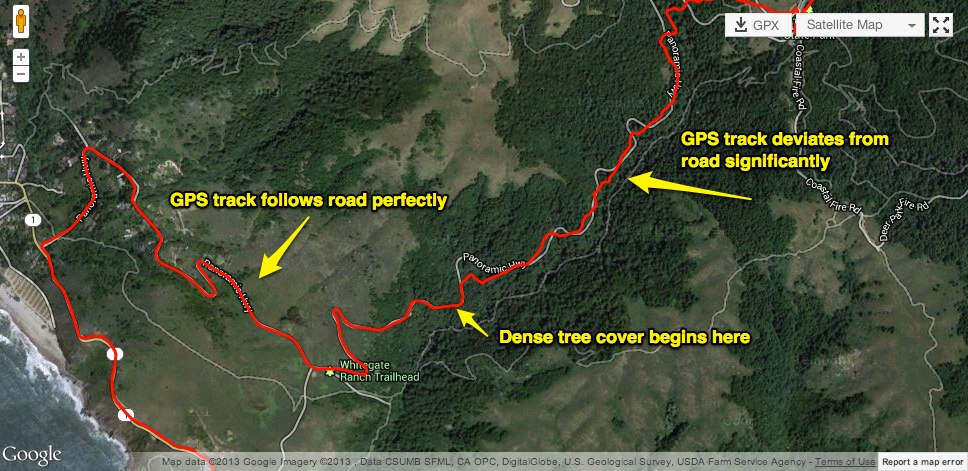
\includegraphics[width=\textwidth]{fig/Afwijkingen&Analyses/Crooked Routes/GPS-Drift_onlnie.jpg}
        \caption{Voorbeeld van gps-drift op een satellietkaart, veroorzaakt door dichte boomgroei~\cite{BadGPSDa19:online}}
    \end{subfigure}
    \caption{Voorbeelden van gps-drift}\label{fig:gps_drift}
\end{figure}

Gps-bouncing is een fenomeen hoofdzakelijk veroorzaakt door hoge gebouwen. Het
\ac{gps}-signaal zal hierbij weerkaatsen tussen de gebouwen, op weg naar het
toestel vanaf de satelliet. De vertraging zorgt er voor dat het apparaat denkt
een extra afstand afgelegd te hebben, terwijl dit niet zo is. De uitkomst van
het traject is dan onvoorspelbaar, wat leidt tot een `cluster' van
\ac{gps}-punten wanneer dit voor een paar punten in dezelfde omgeving gebeurt.
Voorbeelden hiervan zijn terug te vinden op Figuur~\ref{fig:gps_bounce}. Om dit
fenomeen op zijn beurt tegen te gaan, is het best om smoothing toe te passen
bij het berekenen.
\begin{figure}
    \centering
    \begin{subfigure}[b]{0.49\textwidth}
        \centering
        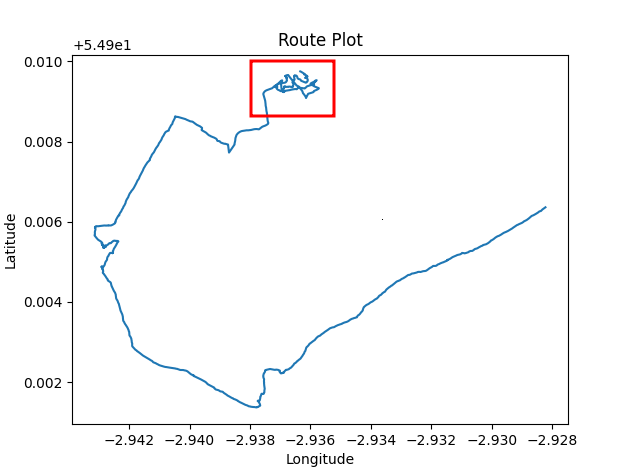
\includegraphics[width=\textwidth]{fig/Afwijkingen&Analyses/Crooked Routes/Crooked GPS Route_Cart.png}
    \end{subfigure}
    \begin{subfigure}[b]{0.49\textwidth}
        \centering
        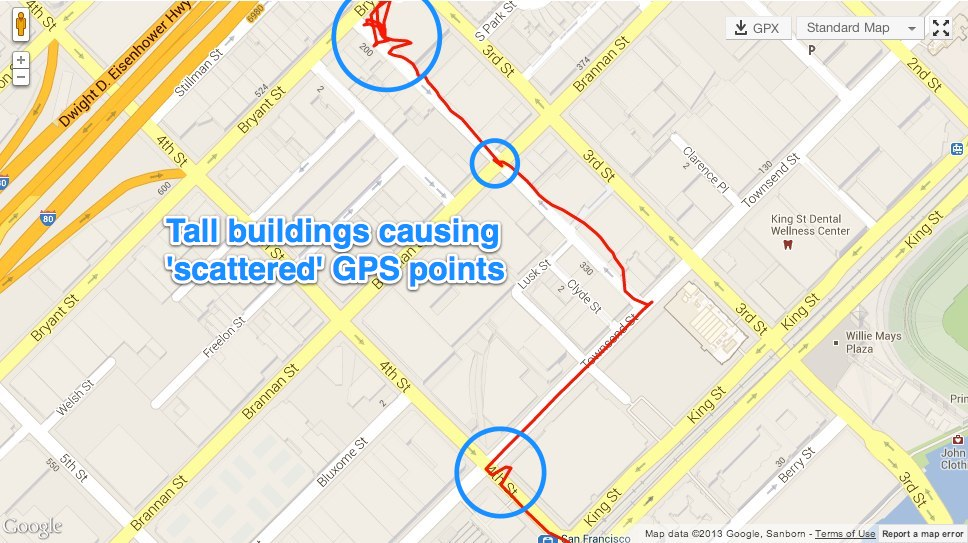
\includegraphics[width=\textwidth]{fig/Afwijkingen&Analyses/Crooked Routes/GPS_bounce_map.jpg}
    \end{subfigure}
    \caption{Voorbeelden van gps-bounce~\cite{BadGPSDa19:online}}\label{fig:gps_bounce}
\end{figure}

Er zijn ook voorbeelden waarbij beide fenomenen voorkomen, zoals te zien is op
Figuur~\ref{fig:gps_drift_bounce_Strava}. Indien we in dit geval op een naïve
manier de totale afgelegde afstand berekenen zal zich een significant verschil
voordoen tussen de afstand die de gebruiker werkelijk afgelegd heeft, en de
berekende afstand. De naïve manier van afstandsberekeningen houdt in dat we de
totale som van het afstandsverschil tussen twee opeenvolgende punten nemen.
\begin{figure}
    \centering
    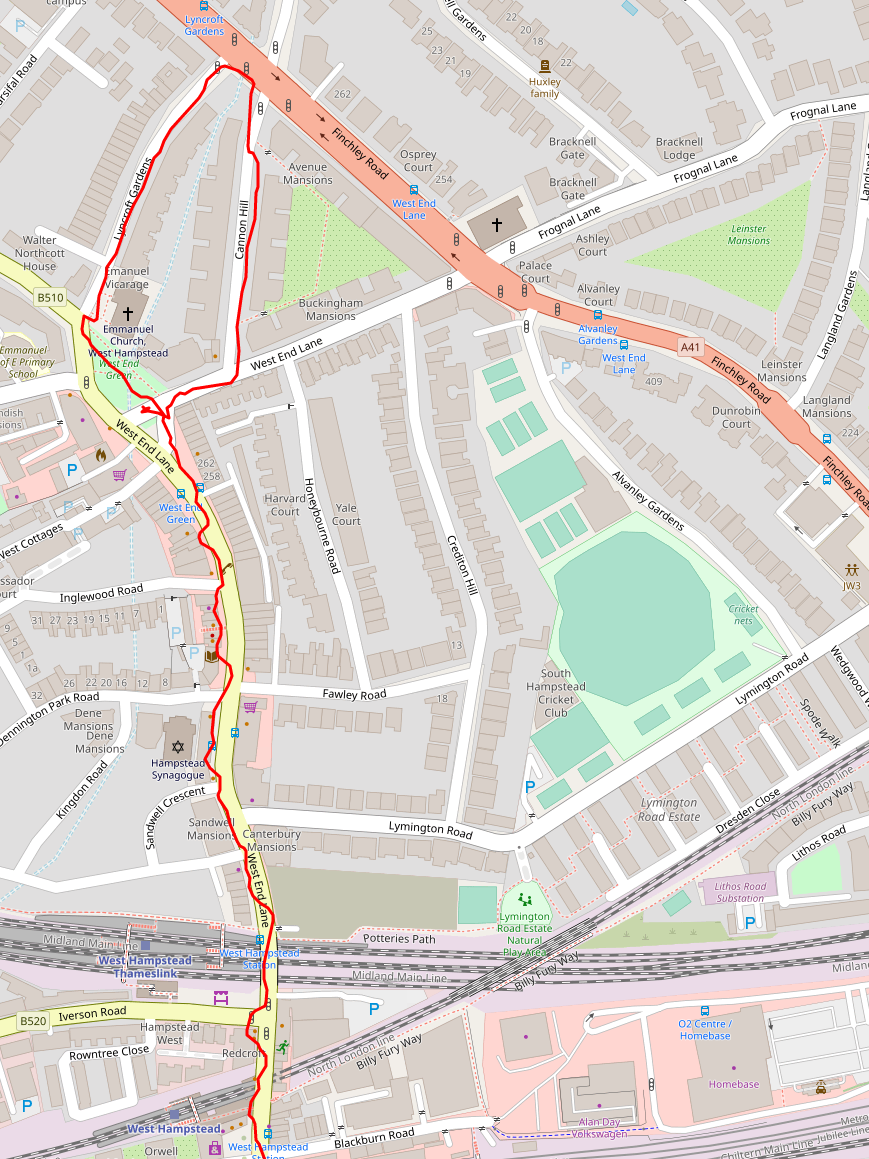
\includegraphics[width=0.7\textwidth]{fig/Afwijkingen&Analyses/Crooked Routes/1_notSnapped.png}
    \caption{Voorbeeld van zowel gps-drift en gps-bounce uit de gebruikte dataset}\label{fig:gps_drift_bounce_Strava}
\end{figure}

Een laatste fenomeen dat kan optreden is \ac{gps}-signal loss. Hierbij gaat het
signaal van de gebruiker verloren, en wordt pas op een later tijdstip terug een
nieuw signaal ontvangen, waardoor een sprong werd gemaakt. In dit geval zou map
matching opnieuw een goede oplossing om dit tegen te gaan. Een tweede oorzaak
die kan leiden tot signal loss, die zeker van toepassing is bij fitness
trackers, is de mogelijkheid tot het pauzeren van een activiteit. In dit geval
wordt de activiteit gepauzeerd voor een bepaald tijdsframe, en wordt er geen
data meer verzameld. Wanneer de activiteit terug wordt hervat, zal er een
sprong zijn in de \ac{gps}-locaties, wat kan leiden tot een verkeerde
berekening van de afstand. In het geval van een pauze zal map matching geen
oplossing zijn, maar zullen we deze `sprongafstand' best weglaten in de
berekeningen. Een voorbeeld hiervan is terug te vinden op
Figuur~\ref{fig:gps_signal_loss}.
\begin{figure}
    \begin{subfigure}[b]{0.49\textwidth}
        \centering
        \includegraphics[width=\textwidth]{fig/Afwijkingen&Analyses/Crooked Routes/1_Full_withArrow.png}
    \end{subfigure}
    \begin{subfigure}[b]{0.49\textwidth}
        \centering
        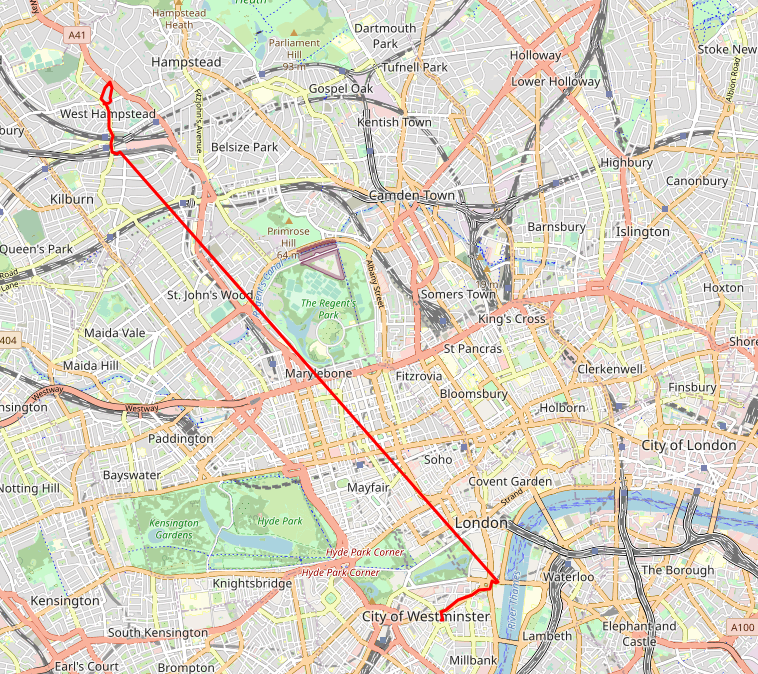
\includegraphics[width=\textwidth]{fig/Afwijkingen&Analyses/Crooked Routes/1_Full_original.png}
    \end{subfigure}
    \caption{Voorbeeld van signal loss uit de gebruikte dataset}\label{fig:gps_signal_loss}
\end{figure}

Een tweede belangrijke maatregel is het gebruik van de de \acp{EPZ}.

\section{Literatuur}
In het verleden is al wat onderzoek verricht in de richting van de
doeltreffendheid van \acp{EPZ} bij fitnesstrackers. Hassan et al. (2018)
beschreven een implementatie van EPZ waarbij het centrum van de zone de
gevoelige locatie is~\cite{sec18has3:online}. Met andere woorden om deze
gevoelige locatie te achterhalen is het dus voldoende deze zone te
identificeren. In tegenstelling tot deze thesis, wordt ervan uitgegaan dat het
centrum geen translatie ondervindt, en er dus geen spatial cloaking wordt
toegepast. In deze paper van~\citeauthor{sec18has3:online} wordt gefocust op de
reconstructie van de cirkel op basis van 3 punten op de rand, wat te zien is op
Figuur~\ref{fig:Hassan_EPZ}. Deze 3 randpunten worden dus bekomen door begin-
of eindpunten te nemen van activiteiten, volgens het perspectief van gebruiker
die geen eigenaar is. Deze begin- of eindpunten zullen zich altijd op de rand
van de cirkel bevinden. Door dit aanvalsmodel toe te passen bekwamen Hassan et
al.\ een succes rate tot 95.1\%. Spatial cloaking werd er aangehaald als
mogelijke verdediging tegen dit soort aanvallen.
\begin{figure}[h]
    \centering
    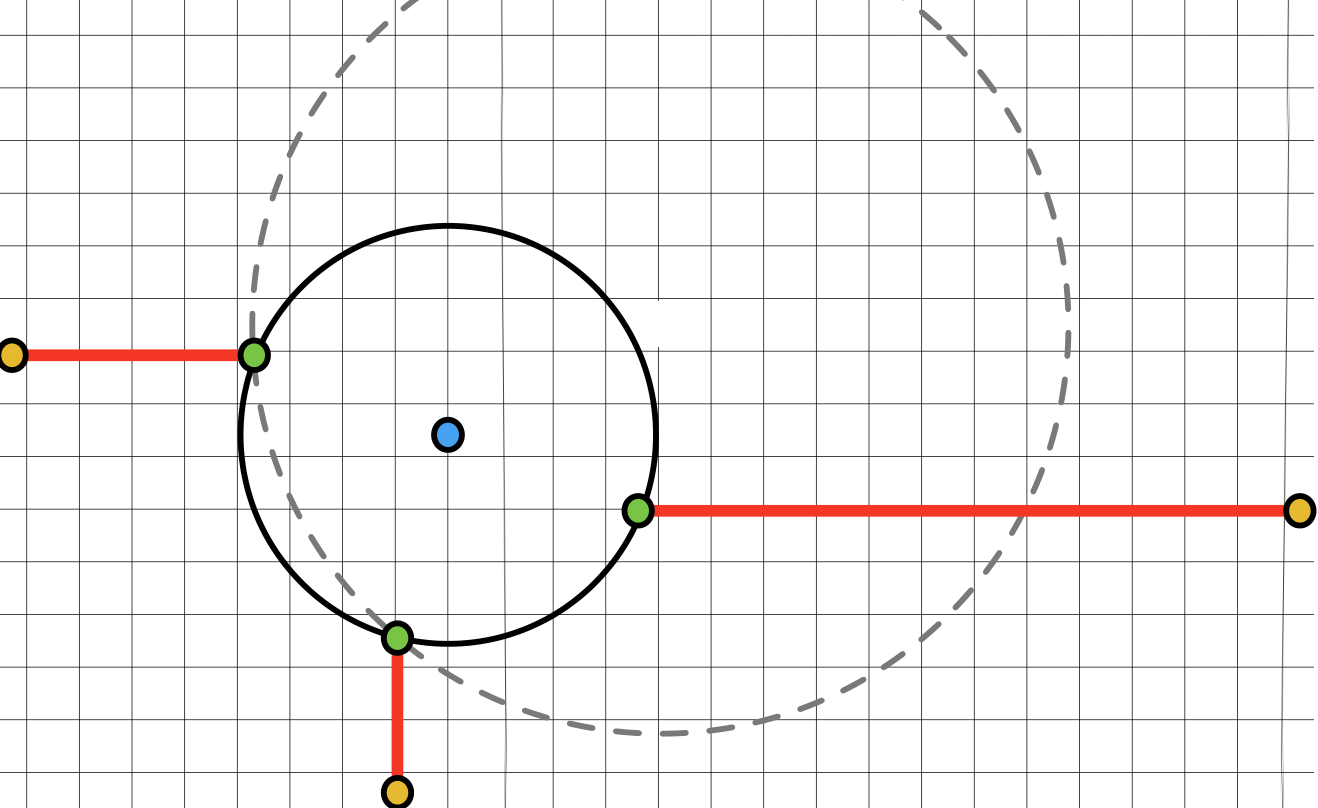
\includegraphics[width=0.6\textwidth]{fig/EPZ-mechanisme/Hassan.png}
    \caption{Mechanisme EPZ beschreven door Hassan et al.~\cite{sec18has3:online}}\label{fig:Hassan_EPZ}
\end{figure}

Een onderzoek door~\citeauthor{10.1145/3491102.3502136} (2022) toonde ook aan
dat heel wat mensen in staat zijn om de gevoelige locatie te achterhalen op
basis van hun intuïtie~\cite{10.1145/3491102.3502136}. Dit gebeurde op basis
van enquêtes die werden afgenomen bij gebruikers van het platform. Deelnemers
aan de enquête moesten op basis van activiteiten opgenomen door een
fitnesstracker, die verhuld waren gebruik makend van een \ac{EPZ}, weliswaar
zonder spatial cloaking, de startlocatie van een gebruiker proberen te
achterhalen. Uit het onderzoek bleek dat 68\% van de ondervraagden bij een
\ac{EPZ}-radius van 200m de beschermde locatie tot op 50m nauwkeurig konden
voorspellen. Hoe meer activiteiten ter beschikking zijn, hoe effectiever de
deelnemers de locatie konden schatten. Deze resultaten op zich zijn alarmerend,
en tonen aan dat \acp{EPZ} verre van perfect zijn, en ook te omzeilen zijn door
een persoon die geen technische achtergrond heeft.

Dhondt et al. (2022) voerden tevens ook een studie naar de mogelijke lekken
aanwezig in het principe van \acp{EPZ}~\cite{Dhondt}. Er wordt in deze paper
een nadruk gelegd op de translatie van de \ac{EPZ}, en hoe deze de privacy van
een gebruiker verhoogt. Ze beschrijven een inferentieaanval die gebruikmaakt
van de totale afstand die terug te vinden bij de activiteit. Het principe van
deze inferentieaanval wordt uitvoerig beschreven in
Hoofdstuk~\ref{chap:inferentieaanval}. In het kort werkt de aanval als volgt:
aan de hand van de totale afgelegde afstand in combinatie met het wegennetwerk
in die omgeving, wordt een poging gedaan om alle mogelijke routes die de
sporter binnenin de \ac{EPZ} zou kunnen afgelegd hebben te reconstrueren. Dit
gebeurt voor elke activiteit. Wanneer dit gedaan wordt voor verschillende
trajecten, kan een locatie voorspeld worden die het meest waarschijnlijk wordt
geacht om de gevoelige locatie te zijn.

Dhondt et al.\ toonden aan dat de beschreven countermeasures door Hassan et
al.\ niet feilloos zijn, en dat deze te omzeilen valt met een successrate van
85\%. Aangezien activiteiten nog steeds totale afstanden van een volledige
route vrijgeven, kunnen ze de afstand afgelegd binnenin de EPZ infereren. Deze
data ligt dan ook aan de grond van de inferentieaanval volgens Dhondt et al.

Het meest recente werk in dit domein is de thesis van
\citeauthor{Verdonck_2022} (2022)~\cite{Verdonck_2022}. Deze thesis bouwt in
grote mate verder op de paper van \citeauthor{Dhondt}, maar maakt gebruik van
alternatieve data.\ \citeauthor{Verdonck_2022} onderzoekt in hoeverre hij
gelijkaardige resultaten kan bekomen door het gebruik van hoogtedata om
beschermde locaties te achterhalen. Via de kennis van hoogtedata van het
stratenplan kan hij via de gekende hoogteverschillen een inferentieaanval
opzetten, die nu geen afstanden maar hoogteverschillen infereerd. Op deze
manier bekomt~\citeauthor{Verdonck_2022} een succes rate van 36\%. Dit lagere
succesratio is terug te brengen naar het feit dat hoogtedata een stuk minder
precies zijn. Ook is hoogtetoename in heel wat regios niet zo significant, wat
de succesrate niet ten goeie komt.

